%%MaD.tex - Notes taken for Materials and Devices Lecture
%%Author: Andy Goetz
%%Date Modified: 10-7-09
%%License: Ask me before reproducing/modifying, etc.


\documentclass{article}

%Make sure you have the file ShumanNote.scy in the same directory as
%this one. It has contains the style sheet for ECE111, and is needed
%to standardize the layout of LateX documents created for the class.
\usepackage{ShumanNotes} 
\usepackage{multirow}
\usepackage{tikz}
\usepackage{program}
\usepackage{listings}
\pdfpagewidth 8.5in 
\pdfpageheight 11in

%This package is used to line up pictures 
\usepackage{graphicx}
\usepackage{fancyvrb}
\usepackage{listings}
%allows cursive font
%\usepackage{amsmath}

%allows hyperlinks 
%\usepackage{hyperref}

\newcommand{\HRule}{\rule{\linewidth}{0.5mm}} 

\lhead{T-16 Test Plan}

\begin{document}

%% These commands allow me to use cursive letter for things such as
%% length.  Note that on ubuntu linux, this required installation of
%% the package 'texlive-fonts-extra'. 
%% Taken from
%% http://www.latex-community.org/forum/viewtopic.php?f=5&t=1404&start=0
\newenvironment{frcseries}{\fontfamily{frc}\selectfont}{}
\newcommand{\textfrc}[1]{{\frcseries#1}}
\newcommand{\mathfrc}[1]{\text{\textfrc{#1}}}

\begin{titlepage}
 
\begin{center}
 
 
\textsc{\LARGE Womprat T-16 Audio Synthesizer}\\[1.5cm]
 
\textsc{\Large Portland State University}\\[0.5cm]
 
 
% Title
\HRule \\[0.4cm]
{ \huge \bfseries Test Plan}\\[0.4cm]
 
\HRule \\[1.5cm]
 
% Author and supervisor
\begin{minipage}{0.4\textwidth}
\begin{center} \large
Andy \textsc{Goetz}, Bradon \textsc{Kanyid}, Jackson \textsc{Pugh}, and Kevin \textsc{Riedl}\\
\end{center}
\end{minipage}

 

 
 
\end{center}
\vfill
{ \textit{} }\\[4.0cm]
\begin{center}
% Bottom of the page
{\large \today}

\end{center} 
\end{titlepage}

\newpage

\textbf{\large Version}
\vspace{.1in}

\begin{tabular}{|p{1in}|p{4in}|p{1in}|}
\hline
\multicolumn{3}{|l|}{\textbf{Document Review}} \\ 
\hline
\textbf{Version}& \textbf{Comments} & \textbf{Date} \\ 
\hline
\textbf{1.0} & Initial release. & 11/24/12 \\
\hline
\end{tabular}

\newpage

\section{Overview}

The T-16 Audio Synthesizer is designed to generate an audio output based on multiple channel inputs, as well as tuneable parameters that are controllable from the user interface.  The functionality can be broken down into several independent sub-modules.  These include a microcontroller to synthesize the audio signal, as well as act as a central communications hub for the other sub-modules, a regulated power supply, an EEPROM memory to dynamically store and load pre-defined user settings and miscellaneous data, an LCD to present the user interface, a DAC to convert the synthesizer's digital audio samples into an analog audio output, and an audio amplifier to provide more output power to an internal speaker and offer a master volume control. 

\centerimage{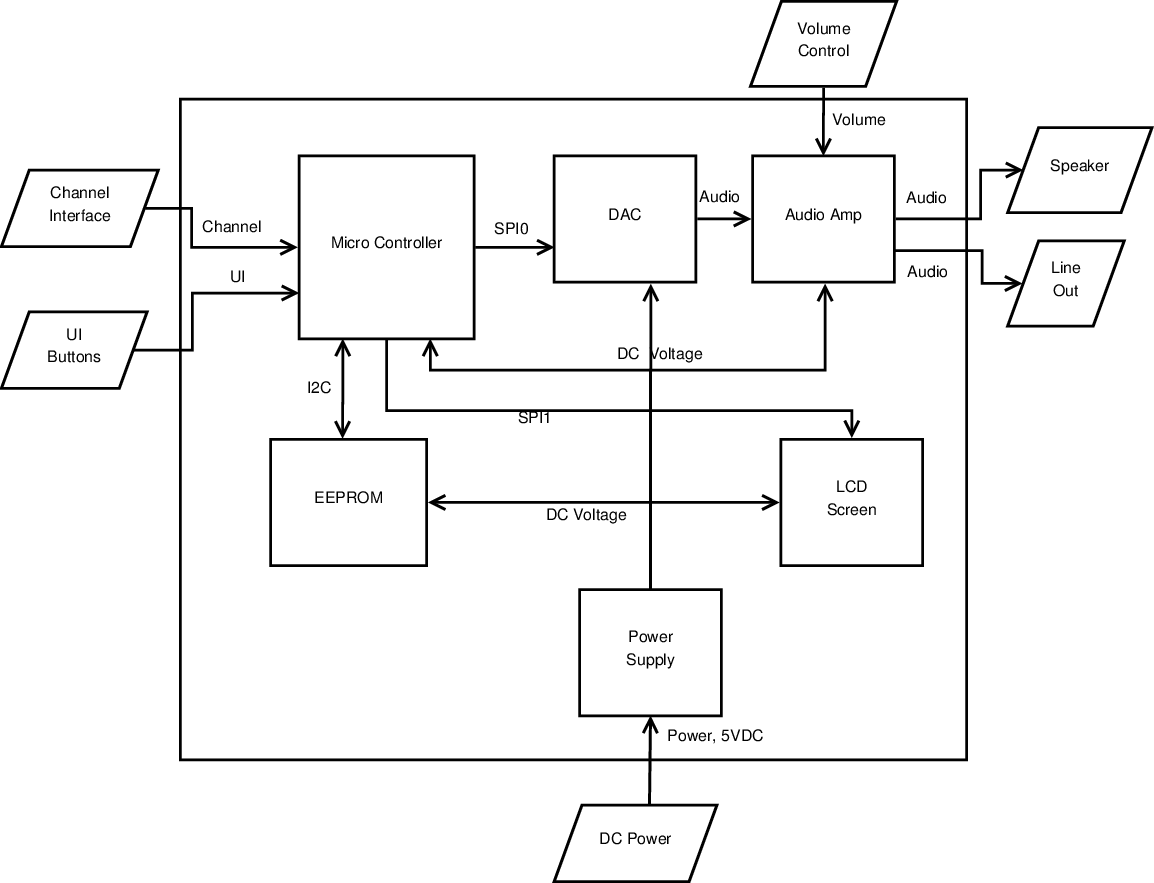
\includegraphics[width=5in]{synth1.png}}{Level 1 Diagram}{fullone}

This document outlines the test approach for the T-16 amplifier. It is
broken down into unit tests, as well as integration and acceptance
tests.

\section{Unit Tests}
\subsection{LCD Tests}
\centerimage{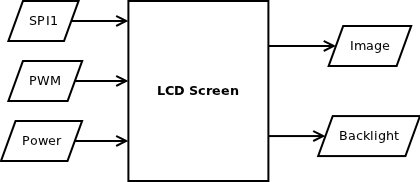
\includegraphics[width=3in]{lcd.png}}{Level 0 Diagram}{LCD}

\begin{tabular}{|p{1in}|p{5in}|}
\hline
\textbf{Module} & LCD \\
\hline
\textbf{Inputs}& SPI: Receives image data from microcontroller.\\
	     & PWM: Backlight brightness control 0-100\% duty cycle.\\
	     & Power: 3.3 VDC Power.\\
\hline
\textbf{Outputs}& Image: Black and white image on 102x64 raster LCD.\\
	      & Backlight: LED light to illuminate the LCD.\\ 
\hline
\textbf{Functionality}& Display the user interface and state of the synthesizer.\\
\hline
\end{tabular}

\subsubsection{UI Overview}
The purpose of the UI is to provide an interface to display the synthesizer's current state and modify the parameters that control the synthesizer state and mapping of the physical channel interface to virtual instruments. 
\subsubsection{Required Equipment}
\begin{itemize}
\item Audio synth board
\item DC Lab Power Supply
\item LCD Daughterboard
\end{itemize}
\subsubsection{Button Test}
The button test verifies that each button state (button up/button down) related to the UI (Up/Down/Left/Right/Ok/Aux) is properly being detected by the CPU. This can be seen through the debug menu, which is entered by powering up while holding any button down. 
\subsubsection{LCD Test}
The LCD test verifies that the LCD is able to display all LCD memory contents and is physically working. This is available via the debug menu, which is entered by powering up while holding any button down.

\subsection{Power Supply Tests}
\centerimage{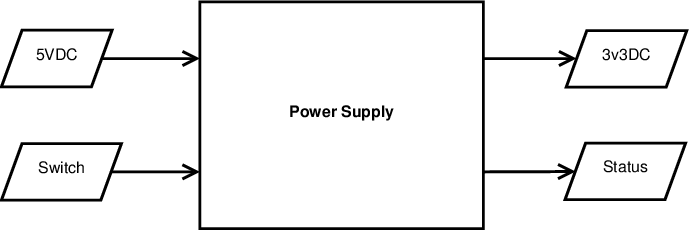
\includegraphics[width=3in]{pwrsply.png}}{Level 0 Diagram}{PSU}

\begin{tabular}{|p{1in}|p{5in}|}
\hline
\textbf{Module} & Power Supply \\
\hline
\textbf{Inputs}& 5VDC: Unregulated power from 5 VDC wall-wart power supply.\\
	     & Switch: On/Off Power Switch.\\
\hline
\textbf{Outputs}& 3v3DC: Regulated 3.3 VDC Power.\\
	      & Status: LED to display if the input power is available.\\ 
\hline
\textbf{Functionality}& The power supply provides regulated 3.3 VDC power to all the subsystems of the audio synthesizer.\\
\hline
\end{tabular}

\subsubsection{Power Supply Overview}
The purpose of the power supply is to provide a constant, regulated 3.3 VDC power to the audio synthesizer subcomponents.  It includes a 2A protection fuse to prevent any high current damage.
\subsubsection{Required Equipment}
\begin{itemize}
\item Audio synth board
\item DC Lab Power Supply
\item Oscilloscope
\end{itemize}
\subsubsection{Fuse Test}
The fuse test verifies that the power supply will burn the fuse and stop supplying power if the current is greater than 2A.  
\subsubsection{Voltage Ripple Test}
The voltage ripple test determines the amount of ripple generated from the output of the power supply.  

\newpage
\subsection{EEPROM Tests}
\centerimage{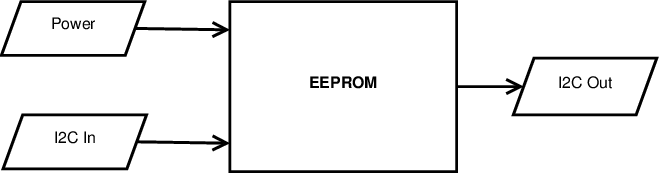
\includegraphics[width=3in]{eeprom.png}}{Level 0 Diagram}{eeprom}

\begin{tabular}{|p{1in}|p{5in}|}
\hline
\textbf{Module} & EEPROM \\
\hline
\textbf{Inputs}& Power: 3.3 VDC Power\\
	     & I2C In: Read data from microcontroller \\
\hline
\textbf{Outputs}& I2C Out: Write data to microcontroller \\ 
\hline
\textbf{Functionality}& Holds user settings for the synthesizer state, as well as the Womprats logo for startup\\
\hline
\end{tabular}
\subsubsection{EEPROM Overview}
The purpose of the EEPROM is to store non-volatile memory so that the Microcontroller can keep settings and store the logo data between power cycles. The Microcontroller talks to the EEPROM via I$^2$C through either burst or byte reads and writes.
\subsubsection{Required Equipment}
\begin{itemize}
\item Audio synth board
\item JTAG programmer for Microcontroller
\end{itemize}
\subsubsection{Read/Write Byte Test}
This test will use the byte write command to write, then use the read byte command to read from the same address. Then, compare the value written to the value read to ensure they are the equal.
\subsubsection{Read/Write Burst Test}
This test will use the burst write command to write a full burst length (16 bytes) to the EEPROM. Then, do a burst read command at the same address. Compare value written with value read to ensure they are equal.

\subsection{Microcontroller Tests}
\centerimage{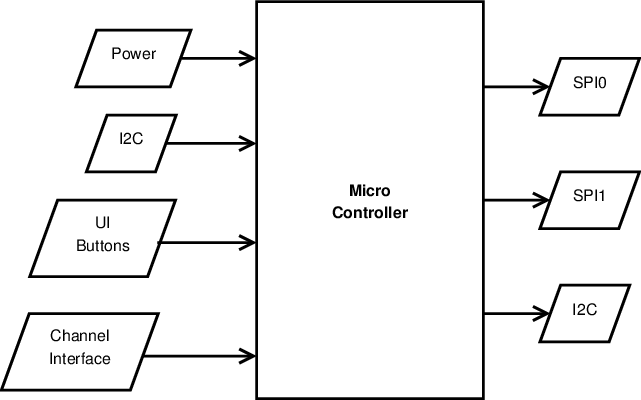
\includegraphics[width=3in]{microcont.png}}{Level 0 Diagram}{micro}

\begin{tabular}{|p{1in}|p{5in}|}
\hline
\textbf{Module} & Microcontroller \\
\hline
\textbf{Inputs}& Power: 3.3 VDC Power\\
	     & I2C: Retrieve data stored in EEPROM\\
	     & UI Buttons: Up/Down/Left/Right/OK/Aux button controls for UI menu interface and entering audio synthesizer settings.\\
	     & Channel Interface: Six analog and digital signal lines that supply parameter control to the audio synthesizer.\\
\hline
\textbf{Outputs}& SPI$_0$: Send digital audio samples to DAC.\\
	      & SPI$_1$: Send image data to LCD.\\
	      & I2C: Store data in EEPROM.\\ 
\hline
\textbf{Functionality}& Implements a software synthesizer that generates an audio signal, shows it's current settings via an LCD screen, is controllable through tunable parameters in the UI and from analog/digital signals on its channel inputs. The tunable parameters are stored in an EEPROM memory that is recalled on startup.\\
\hline
\end{tabular}

\subsubsection{Microcontroller Overview}
The microcontroller used in the T-16 audio synthesizer is an NXP
LPC1114. It is an arm Cortex M0 microcontroller.

\subsubsection{Equipment Required}
\begin{itemize}
  \item T-16 synthesizer board
  \item JTAG Programmer
  \item CodeRed Development Environment 
\end{itemize}

\subsubsection{Programming Test} 
The T-16 audio synthesizer must be able to be programmed via its JTAG port. 

\subsubsection{Diagnostic Test}
The Diagnostic LEDs of the microcontroller must be blinked, to
demonstrate that the test code works.

\subsection{DAC Tests}
\centerimage{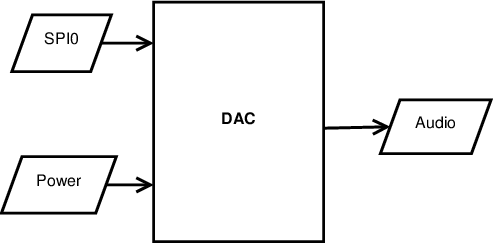
\includegraphics[width=3in]{dac.png}}{Level 0 Diagram}{dac}

\begin{tabular}{|p{1in}|p{5in}|}
\hline
\textbf{Module} & DAC \\
\hline
\textbf{Inputs}& SPI$_0$: Audio samples received from the microcontroller\\
	     & Power: 3.3 VDC power\\
\hline
\textbf{Outputs}& Audio: 0-3.3V audio signal \\ 
\hline
\textbf{Functionality}& The DAC takes the digital audio sample from the microcontroller and converts an analog 0-3.3V audio signal.\\
\hline
\end{tabular}

\subsubsection{DAC Overview}
The DAC used in the T-16 audio synthesizer is controlled by a SPI
interface. It takes a 12bit value from the microcontroller, and
converts it into an analog value from 0 to 3.3 volts. It important
that the microcontroller can output values to the SPI DAC. 

\subsubsection{Required Equipment}
\begin{itemize}
  \item T-16 Audio Synthesizer Board
  \item Oscilloscope
  \item 5 volt DC power supply
\end{itemize}

\subsubsection{DAC Test}
The microcontroller must be able to output a simple sawtooth signal to
the DAC, visible on its output signal.

\subsection{Audio Amplifier Tests}
\centerimage{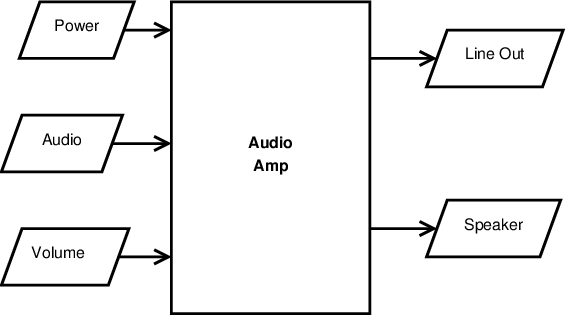
\includegraphics[width=3in]{audioamp.png}}{Level 0 Diagram}{audio}

\begin{tabular}{|p{1in}|p{5in}|}
\hline
\textbf{Module} & Audio Amplifier \\
\hline
\textbf{Inputs} & Power: 3.3 VDC Power\\
	      & Audio: 0-3.3V audio signal from DAC\\
	      & Volume: Controls the audio output volume. Logarithmic control.\\
\hline
\textbf{Outputs}& Line out: Unamplified audio output to external line-out.\\ 
	      & Speaker: Amplified audio output to internal speaker.\\
\hline
\textbf{Functionality}& Provide an amplified audio out that can be heard over the internal speaker or line-out to an external audio device.\\
\hline
\end{tabular}
\subsubsection{Audio Amplifier Overview}
The purpose of the audio amplifier is to provide an amplified audio signal to the internal speakers or a line-out to an external audio device.  It receives a 0-3.3 VDC signal and has an external volume control to adjust the output volume.  If the line-out is being used, the internal speaker will turn off.
\subsubsection{Required Equipment}
\begin{itemize}
\item Audio synth board
\item DC Lab Power Supply
\item Oscilloscope
\end{itemize}
\subsubsection{Frequency Test}
The frequency test determines the maximum input audio frequency that can be processed without significant output signal distortion.
\subsubsection{Line-out Test}
The line-out test verifies that the internal speaker turns off when the line-out is in-use.  When the line-out is removed, the internal speaker should turn on again.
\subsubsection{Volume Control Test}
The volume control test verifies the volume knob increases/decreases the output volume of the audio amplifier.  The volume should be off when the knob is twisted in the off position and reach the loudest noise level when the knob is twisted in the fully on position.

\section{Integration Tests}

\subsection{Power-On Self-Test}
The power-on self-test verifies the output power from the power supply is correctly biasing each submodule.  Each submodule will be connected to the power supply and measured to ensure it is operating correctly.

\subsubsection{Required Equipment}
\begin{itemize}
\item Audio synthesizer board
\item Wall-wart for synth board
\item JTAG programmer for Microcontroller
\end{itemize}

\subsection{DAC-Audio Amplifier Test}
The DAC-audio amplifier test verifies the DAC feeds the proper input values to the audio amplifier.  The audio amplifier should playback the correct analog input signal without any new artifacts or distortions.
\subsubsection{Required Equipment}
\begin{itemize}
\item Audio synthesizer board
\item Wall-wart for synth board
\item JTAG programmer for Microcontroller
\end{itemize}

\subsection{Display Womprat on LCD screen}
The purpose of this test is to ensure that the interface between the EEPROM, the Microcontroller, and the LCD daughterboard work properly. The test involves reading the Womprat logo from the EEPROM into the Microcontroller and then sending the logo data to the LCD screen to display the logo. This will test the I$^2$C driver for the EEPROM, the SPI driver for the LCD screen, and also will ensure that the hardware involved is functional.
\subsubsection{Required Equipment}
\begin{itemize}
\item Audio synthesizer board
\item Wall-wart for synth board
\item LCD daughter board
\item JTAG programmer for Microcontroller
\end{itemize}

\newpage
\section{Acceptance Tests}
The primary goal of the T-16 audio amplifier is to demonstrate the
engineering skills of its team members in an interview
situation. Several acceptance tests have been outlined below:

\subsection{Temperature Test}
The completed T-16 Synthesizer must not rise above $10^\circ$ Celsius
while the internal amplifier is in use.
\subsection{Untrained User}
	The purpse of this test is to make sure that the finished product is easy
	for an untrained person to pick up and start using. The maximum amount of
	time they should take to figure out how it works is 5 minutes.

\section {Test Forms}
\subsection {Integration Tests}
\begin{tabular}{|p{1.3in}|p{3in}|p{.8in}|p{.5in}|}
  \hline
  \textbf{Test Case Name:} & Display Womprat on LCD screen & \textbf{Test ID \#:} & 1\\
  \hline
  \textbf{Description:} &
The purpose of this test is to ensure that the interface between the EEPROM, the Microcontroller, and the LCD daughterboard work properly. The test involves reading the Womprat logo from the EEPROM into the Microcontroller and then sending the logo data to the LCD screen to display the logo. This will test the I$^2$C driver for the EEPROM, the SPI driver for the LCD screen, and also will ensure that the hardware involved is functional.
  & \textbf{Type:} & whitebox \\
  \hline
  \multicolumn{4}{|l|}{\textbf{Tester Information}} \\ 
  \hline
  \textbf{Name of Tester:} & Kevin Riedl& \textbf{Date:} & \\
  \hline
  \textbf{Hardware Ver:} & T-16 v1.0 & \textbf{Time:} & \\
  \hline
  \textbf{Setup:} & \multicolumn{3}{|p{4.3in}|}{Properly powered Audio synth board plugged into LCD daughter board and JTAG} \\
  \hline
\end{tabular}
\begin{tabular}{|p{.3in}|p{1.1in}|p{1.2in}|p{.25in}|p{.25in}|p{.3in}|p{1.7in}|}
  \hline
  \textbf{Step} & \textbf{Action} & \textbf{Expected Result} & \textbf{Pass} & \textbf{Fail} & \textbf{N/A} & \textbf{Comments} \\
  \hline
  1 & Power Board (switch on) & LCD displaying Womprat logo and startup screen& & & & \\
  \hline
  \multicolumn{3}{|l|} {\textbf{Overall Test result:}}& & & & \\
  \hline
\end{tabular}

\subsection{Unit Tests}
\begin{tabular}{|p{1.3in}|p{3in}|p{.8in}|p{.5in}|}
  \hline
  \textbf{Test Case Name:} & EEPROM Read/Write Byte Test & \textbf{Test ID \#:} & 2\\
  \hline
  \textbf{Description:} &
  This test is to verify that the EEPROM memory is both readable and writeable. To test this, we write a random (known) value to the EEPROM and then attempt to read back this known value. If the values are the same, we know that the memory write and read was successful. We need to do this in a few places in memory to verify that addressing is also working. 
  & \textbf{Type:} & blackbox \\
  \hline
  \multicolumn{4}{|l|}{\textbf{Tester Information}} \\ 
  \hline
  \textbf{Name of Tester:} & Bradon Kanyid & \textbf{Date:} & \\
  \hline
  \textbf{Hardware Ver:} & T-16 v1.0 & \textbf{Time:} & \\
  \hline
  \textbf{Setup:} & \multicolumn{3}{l|}{Properly powered Audio synth board and JTAG interface} \\
  \hline
\end{tabular}
\begin{tabular}{|p{.3in}|p{1.2in}|p{1.2in}|p{.25in}|p{.25in}|p{.3in}|p{1.6in}|}
  \hline
  \textbf{Step} & \textbf{Action} & \textbf{Expected Result} & \textbf{Pass} & \textbf{Fail} & \textbf{N/A} & \textbf{Comments} \\
  \hline
  1 & Write random value to address 000, then read from address 000. & The value read is the same as the value written & & & &\\
  \hline
  2 & Write random value to address FFF, then read from address FFF. & The value read is the same as the value written & & & &\\
  \hline
  3 & Write random value to random address between 000 and FFF, then read back from same address & The value read is the same as the value written & & & &\\
  \hline
  \multicolumn{3}{|l|} {\textbf{Overall Test result:}}& & & & \\
  \hline
\end{tabular}
\newpage

\begin{tabular}{|p{1.3in}|p{3in}|p{.8in}|p{.5in}|}
  \hline
  \textbf{Test Case Name:} & DAC Waveform Test & \textbf{Test ID \#:} & 3\\
  \hline
  \textbf{Description:} &

  The purpose of this test is to verify that the DAC attached to the
  microcontroller can output analog voltages, from 0 to 3.3 volts.

  & \textbf{Type:} & whitebox \\
  \hline
  \multicolumn{4}{|l|}{\textbf{Tester Information}} \\ 
  \hline
  \textbf{Name of Tester:} &  & \textbf{Date:} & \\
  \hline
  \textbf{Hardware Ver:} & T-16 v1.0 & \textbf{Time:} & \\
  \hline
  \textbf{Setup:} & \multicolumn{3}{l|}{Properly powered Audio synth board and JTAG interface} \\
  \hline
\end{tabular}

\begin{tabular}{|p{.3in}|p{1.2in}|p{1.2in}|p{.25in}|p{.25in}|p{.3in}|p{1.6in}|}
  \hline
  \textbf{Step} & \textbf{Action} & \textbf{Expected Result} & \textbf{Pass} & \textbf{Fail} & \textbf{N/A} & \textbf{Comments} \\
  \hline
  1 & Write a small test program to set the output of the DAC to values ranging between 0 and 4095.  &  & & & &\\
  \hline
  2 & Attach an oscilloscope to the VOUT test point of the T-16 circuit board.  & A ramp function should be visible on the oscilloscope.& & & &\\
  \hline
  \multicolumn{3}{|l|} {\textbf{Overall Test result:}}& & & & \\
  \hline
\end{tabular}

\newpage

\subsection{Acceptance Tests}
\begin{tabular}{|p{1.3in}|p{3in}|p{.8in}|p{.5in}|}
  \hline
  \textbf{Test Case Name:} & Untrained User Test & \textbf{Test ID \#:} & 4\\
  \hline
  \textbf{Description:} &

	The purpse of this test is to make sure that the finished product is easy
	for an untrained person to pick up and start using. The maximum amount of
	time they should take to figure out how it works is 5 minutes.

  & \textbf{Type:} & blackbox \\
  \hline
  \multicolumn{4}{|l|}{\textbf{Tester Information}} \\ 
  \hline
  \textbf{Name of Tester:} &  & \textbf{Date:} & \\
  \hline
  \textbf{Hardware Ver:} & T-16 v1.0 & \textbf{Time:} & \\
  \hline
  \textbf{Setup:} & \multicolumn{3}{l|}{Finished Audio synth board in working enclosure and Properly powered} \\
  \hline
\end{tabular}
\begin{tabular}{|p{.3in}|p{1.1in}|p{1.2in}|p{.25in}|p{.25in}|p{.3in}|p{1.7in}|}
  \hline
  \textbf{Step} & \textbf{Action} & \textbf{Expected Result} & \textbf{Pass} & \textbf{Fail} & \textbf{N/A} & \textbf{Comments} \\
  \hline
  1 & Provide untratined user with completed synth & Untrained user will have completed synth & & & &\\
  \hline
  2 & Tell the untrained user to figure out how the synth works and start a 5 minute countdown & User will figure out how the synth works within 5 minutes & & & &\\
  \hline
  \multicolumn{3}{|l|} {\textbf{Overall Test result:}}& & & & \\
  \hline
\end{tabular}

\end{document}
